% !TEX root = ../main.tex
%

\section{Results}

\subsection{Main findings}

Figure \ref{fig::toxicity_aq_stats} shows the mean difference in toxicity and argument quality between each moderation strategy. Discussions where a moderator is absent feature overall significantly increased toxicity and decreased argument quality. Some strategies seem to have both statistically (Kruskal-Wallis $p=0$ for both measures) and qualitatively significant impact on discussions. Our proposed \ac{RL}-inspired strategy (see Section \ref{ssec:setup:strategies}) significantly outperforms all baselines, as well as all other established strategies, by a smaller margin. This is more evident when looking at toxicity. In fact, contrary to our expectations, the strategies based on widely used guidelines do not seem to outperform the baselines (apart from the moderator being absent).

Table \ref{tab:timeseries}\footnote{The size of our dataset allows us to use parametric tests.} shows the effect of each moderation strategy on toxicity and argument quality through the timeframe of the discussion. We observe a negative correlation through time for all moderation strategies, suggesting that all strategies eventually deal to a limited extent with both high toxicity and low argument quality, compared to unmoderated discussions.

Furthermore, as demonstrated by Figure \ref{fig::intervention_count}, \ac{LLM} moderators will respond at almost every point in the discussion. We also observe that \ac{LLM} user-agents are unusually lenient towards repeated, unneeded interventions of moderators, which is not representative of human behavior. In this situation, human users tend to get irritated, and we can usually observe a rise in toxicity \cite{schaffner_community_guidelines, make_reddit_great, proactive_moderation, cresci_pesonalized_interventions}.

\begin{figure*}[t]
    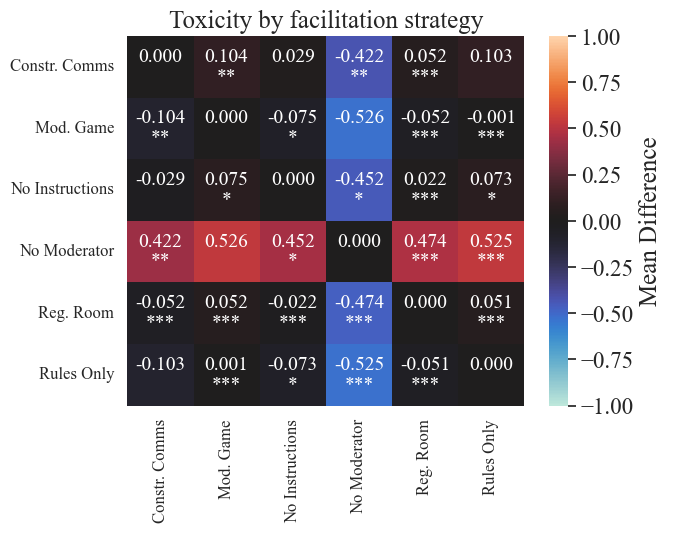
\includegraphics[width=0.48\linewidth]{toxicity_stats.png} \hfill
    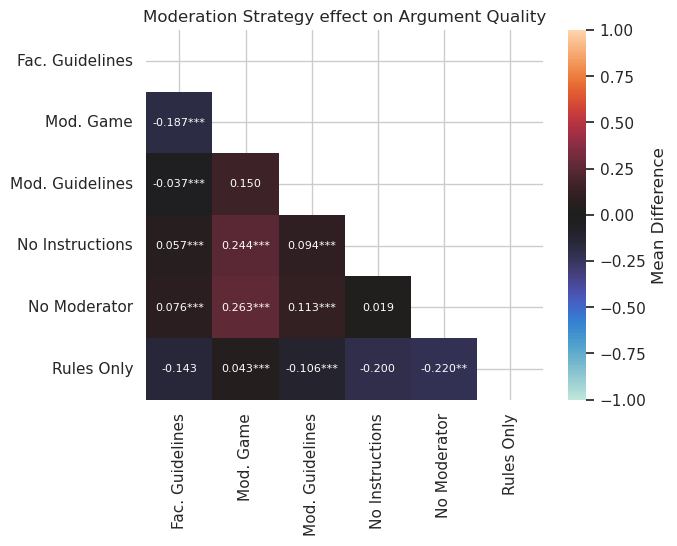
\includegraphics[width=0.48\linewidth]{argumentq_stats.png}
	\centering
	\caption{Mean difference of Toxicity (left) and Argument Quality (right) between each moderation strategy. $A[i, j] = 0.3^{***}$ indicates that the strategy $j$ is better than the strategy $i$ for an average of $0.3$ points with $p<0.001$. Each comparison is accompanied by Dunn's posthoc test for multiple comparisons \cite{dunn}, in the form of significance asterisks.}
	\label{fig::toxicity_aq_stats}
\end{figure*}

\begin{figure}
	\centering
	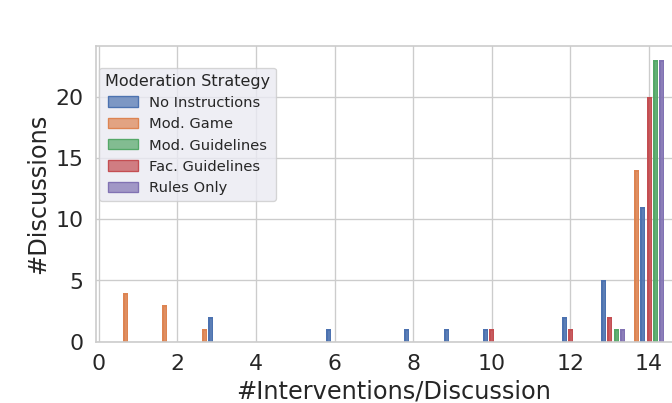
\includegraphics[width=\columnwidth]{intervention_count.png}
	\caption{Histogram of interventions by LLM moderators over all discussions.}
	\label{fig::intervention_count}
\end{figure}

\begin{table}[htbp]
    \centering
    \begin{tabular}{lll}
        \toprule
        \textbf{Variable} & \textbf{Toxicity} & \textbf{Arg.Q.} \\
        \midrule
        Intercept & 2.168\textsuperscript{***} & 2.177\textsuperscript{***} \\
        Fac. Guid. & -0.165\textsuperscript{**} & -0.053 \\
        Mod. Guid. & -0.146\textsuperscript{**} & -0.035 \\
        \ac{RL} Game & -0.346\textsuperscript{***} & -0.286\textsuperscript{***} \\
        No Instructions & -0.325\textsuperscript{***} & -0.183\textsuperscript{***} \\
        Rules Only & -0.493\textsuperscript{***} & -0.382\textsuperscript{***} \\
        time & -0.021\textsuperscript{***} & -0.026\textsuperscript{***} \\
        Fac. Guid:time & -0.018\textsuperscript{***} & -0.003 \\
        Mod. Guid:time & -0.028\textsuperscript{***} & -0.009\textsuperscript{.} \\
        \ac{RL} Game:time & -0.020\textsuperscript{***} & 0.003 \\
        No Instructions:time & 0.007 & 0.019\textsuperscript{***} \\
        Rules Only:time & 0.010\textsuperscript{*} & 0.019\textsuperscript{***} \\
        \bottomrule
    \end{tabular}
    \smallskip
    \small
    \textsuperscript{.} $p<0.1$, \textsuperscript{*} $p<0.05$, \textsuperscript{**} $p<0.01$, \textsuperscript{***} $p<0.001$
    \normalsize
    \caption{OLS Regression Coefficients for Toxicity ($Adj. R^2=0.054$ and Argument Quality ($Adj. R^2=0.019$). \textit{“Time”} denotes dialogue turn, reference factor is \textit{“No moderator”}.}
    \label{tab:timeseries}
\end{table}


\subsection{Ablation study}

We test the effects of our proposed methodology by running $8$ synthetic discussions and comparing their \textit{Diversity} scores (Section \ref{ssec:methodology:diversity}) with our original dataset, as well as with human discussions. We use the Cornell eRulemaking “Regulation Room” dataset \footnote{\url{http://archive.regulationroom.org}. Any opinions, findings, and conclusions or recommendations expressed in this material are those of the author(s) and do not necessarily reflect the views of the CeRI (Cornell e-Rulemaking Initiative).}, from which we extract all comments from all initiatives. We assert that diversity distributions closer to the ones observed in the human discussions indicate they are realistic.


\subsubsection{Models}

The Qwen 2.5 model approximates the human \textit{Diversity} scores the best (Figure \ref{fig::diversity}), followed by the Mistral (abl.) model. The LLaMa 3.1 model performs the worst. This may indicate that models subjected to intense alignment procedures may not be able to replicate human behavior as authentically as other models (as reported in \citet{Park2023GenerativeAI}). Alternatively, LLaMa's longer comments (Figure \ref{fig::comment_length}) may have caused the higher diversity scores (see Section \ref{ssec:results:corr}).

In that case however, we would expect the Mistral model to be the best model at approximating human discussions. This may indicate that abliteration may not be an effective way of getting around alignment, or that this specific model was not properly abliterated. This is further supported by the fact that the abliterated model does not seem to exhibit increased toxicity (Appendix \ref{ssec:appendix:analysis} Figure \ref{fig}).


\subsubsection{Turn taking}

We investigate three turn taking functions: The Round Robin algorithm, which gets each user to talk in a predetermined, unchanging order, random selection, and our proposed turn taking algorithm (Section \ref{ssec:experimental:turn}).

While the turn taking function by itself is not enough to approximate the human discussions (Figure \ref{fig::diversity} — since all the distributions diverge from the human distribution), it still seems to improve synthetic discussions. Discussions where the turn to speak was given either by chance or rotation, demonstrate extremely low diversity scores, diverging significantly from the human diversity distribution. This can not be explained by comment length (Figure \ref{fig::comment_length}).


\subsubsection{Prompting}

We run discussions where user-agents are not assigned (1) \acp{SDB}, (2) roles, (3) are given a baseline prompt (see Appendix \ref{ssec:appendix:prompts} Table \ref{tab:base_prompts}).

Figure \ref{fig::diversity} demonstrates that, while our approach (using roles, \acp{SDB} and the improved instruction prompt) is not enough to create identical discussions with human ones, removing any of its aspects leads to a significant divergence. This divergence is similar to the one observed when changing the turn taking function, and can similarly not be attributed to differences in comment length (Figure \ref{fig::comment_length}).


\subsection{Correlation between discussion size and diversity}
\label{ssec:results:corr}

While there is a statistically significant difference between the two variables in synthetic discussions ($p<.000$), this does not appear to be the case in human discussions ($p=0.668$). Nevertheless, there is a qualitatively significant  ($Adj. R^2=0.196$), positive correlation ($\textit{diversity} = 2.633\mathrm{e}{-05} \times \textit{\#words} \times \textit{is\_synthetic}$).

\begin{figure*}[t]
    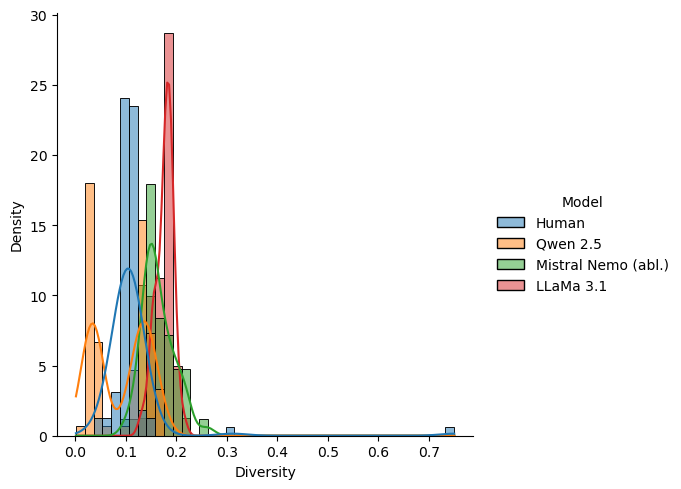
\includegraphics[width=0.30\linewidth]{rougel_model.png} \hfill
    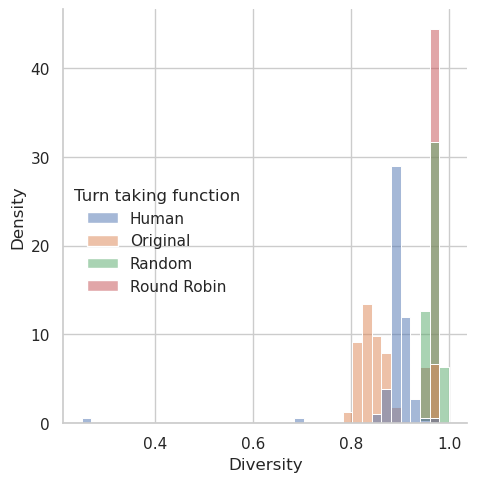
\includegraphics[width=0.30\linewidth]{rougel_turns.png}
    \hfill
    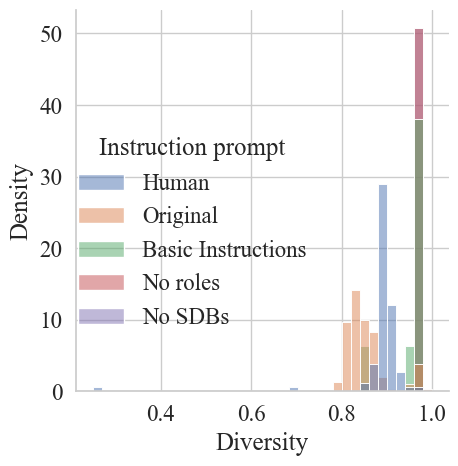
\includegraphics[width=0.30\linewidth]{rougel_prompts.png}
	\centering
	\caption{Diversity (Section \ref{ssec:methodology:diversity}) distribution for each discussion by model (Section \ref{ssec:experimental:model}), turn-taking function $u$ (Section \ref{ssec:experimental:turn}), and prompting function $\phi$ used (Section \ref{ssec:experimental:prompts}).}
	\label{fig::diversity}
\end{figure*}

\begin{figure*}[t]
    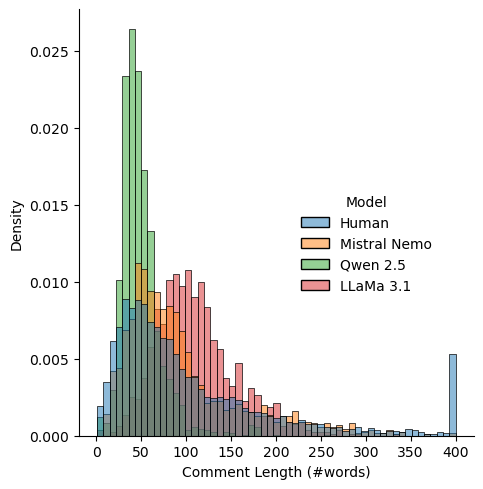
\includegraphics[width=0.30\linewidth]{comment_len_model.png} \hfill
    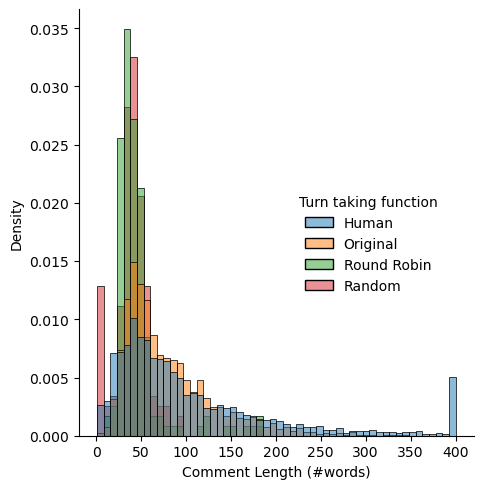
\includegraphics[width=0.30\linewidth]{comment_len_turns.png}
    \hfill
    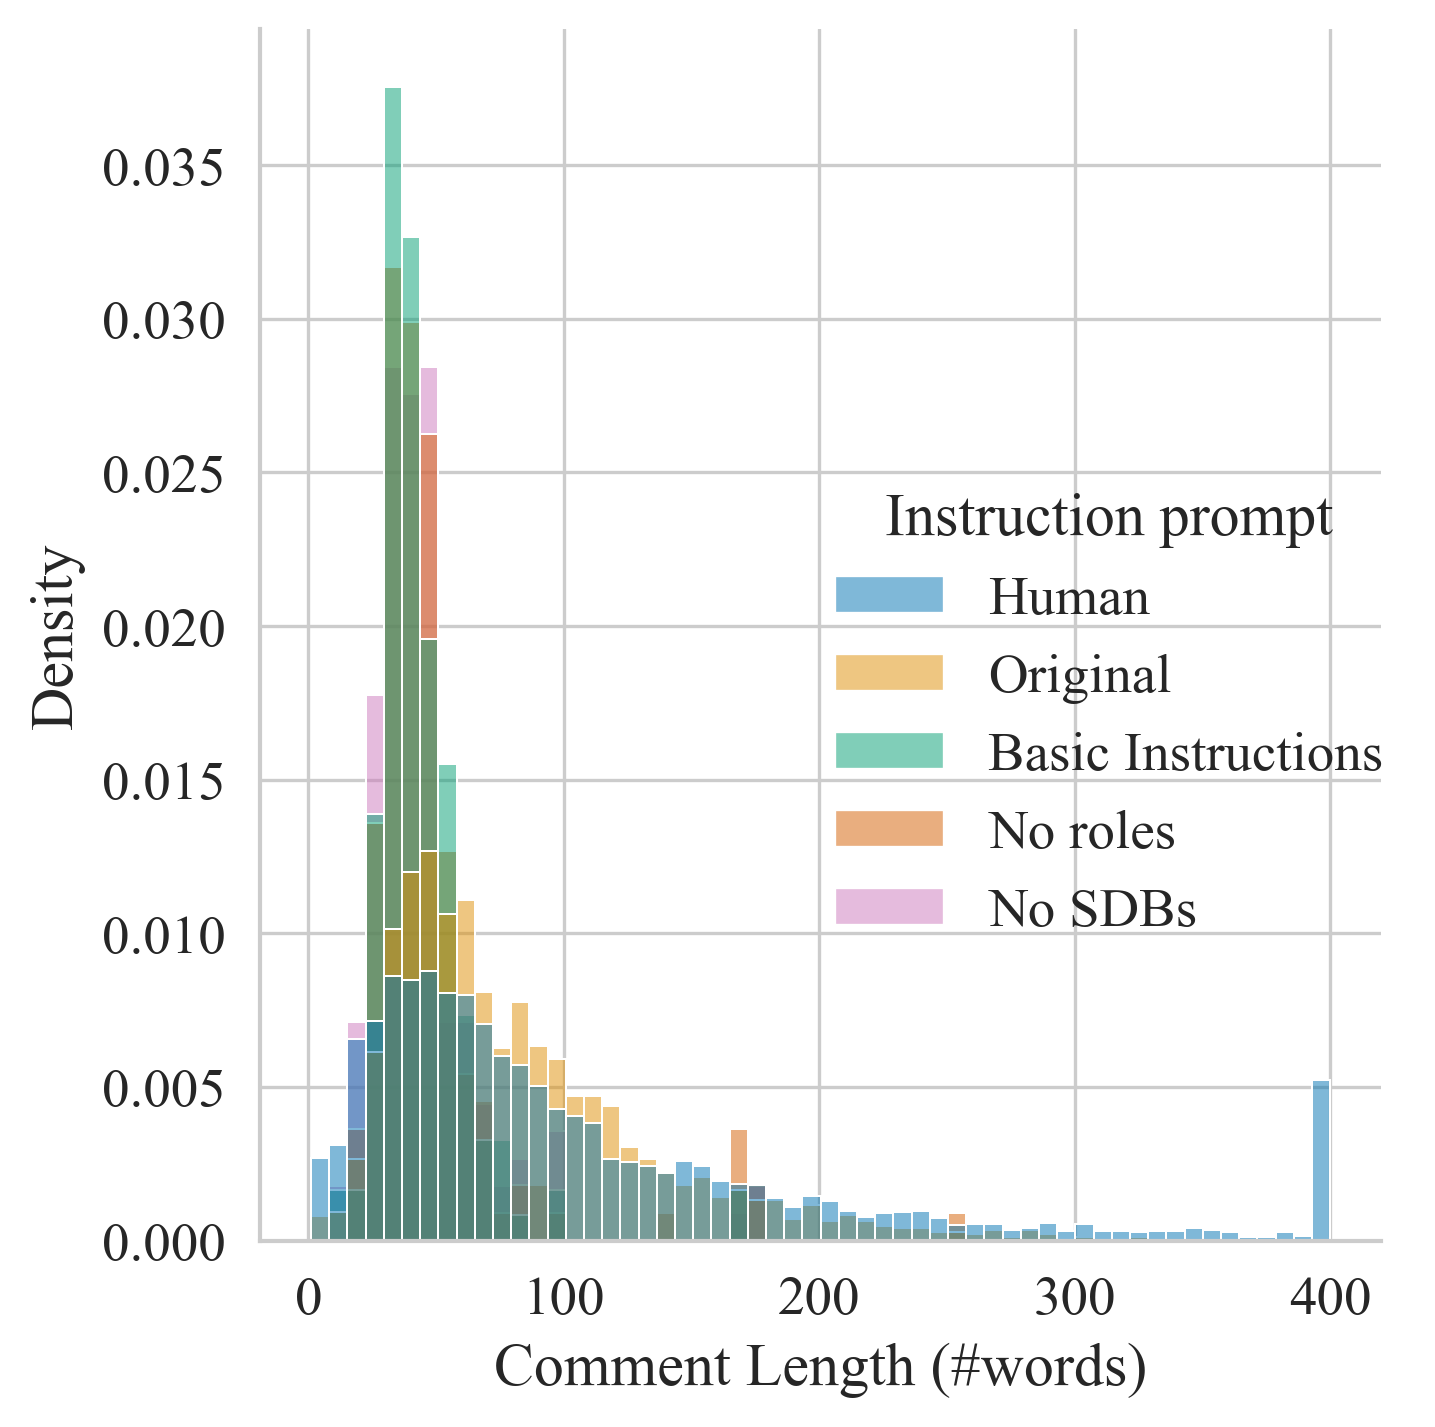
\includegraphics[width=0.30\linewidth]{comment_len_prompts.png}
	\centering
	\caption{Comment length for each discussion by model (Section \ref{ssec:experimental:model}), turn-taking function $u$ (Section \ref{ssec:experimental:turn}), and prompting function $\phi$ used (Section \ref{ssec:experimental:prompts}). For ease of comparison, comments above $400$ words are marked at the end of the x-axis.}
	\label{fig::comment_length}
\end{figure*}



